\documentclass[pdf]{beamer}
\usepackage{lmodern}
\usepackage{hyperref}
\mode<presentation>{\usetheme{PaloAlto}}
\title{Speckle Interferometry}
\author{Matt Rauen and David Fan}
\date{\today}
\begin{document}
\begin{frame}
\titlepage
\end{frame}

\section{Abstract}
\begin{frame}{Abstract}
We used speckle interferometry to image the effect of applying a voltage to a piezo. To do this, we used a beam splitter to create interference between reflected light off of a piezo and a reference object, which generated a speckle pattern. By shifting the reference object and taking images of the speckle pattern with a digital camera, we were able to compute the absolute phase of the points on the piezo, pixel by pixel. By repeating this procedure after applying a voltage, we calculated the phase difference applied by the voltage. We observed a considerable amount of error, which we believe arises from movement of the camera, as well as fluctuations due to atmospheric conditions.
\end{frame}

\section{Research Questions}
\begin{frame}{Research Questions}
\begin{center}
{\bf Primary Question:}

How does the piezo deform when a voltage is applied to it?
\end{center}
More concretely, we want to construct a topological map of the shift at each point, where each point is characterized by the phase difference (relative to the wavelength of light we used) between its original position and its position after the applied voltage.
\begin{figure}[htbp]
\centering
\includegraphics[width=0.3\textwidth]{gaussian_bump.png}
\end{figure}
\end{frame}

\section{Background}
\begin{frame}{Speckle Patterns}
Speckle patterns are generated by interference of a set of wavefronts. In particular, in our experiment, this interference is between light reflected off of the reference object and the object of interest.\\
\vspace{0.3cm}
{\bf Important Property of Speckle Patterns:}
The size of the speckles is inversely proportional to the size of the aperture.
\begin{figure}[!htb]
\minipage{0.3\textwidth}
  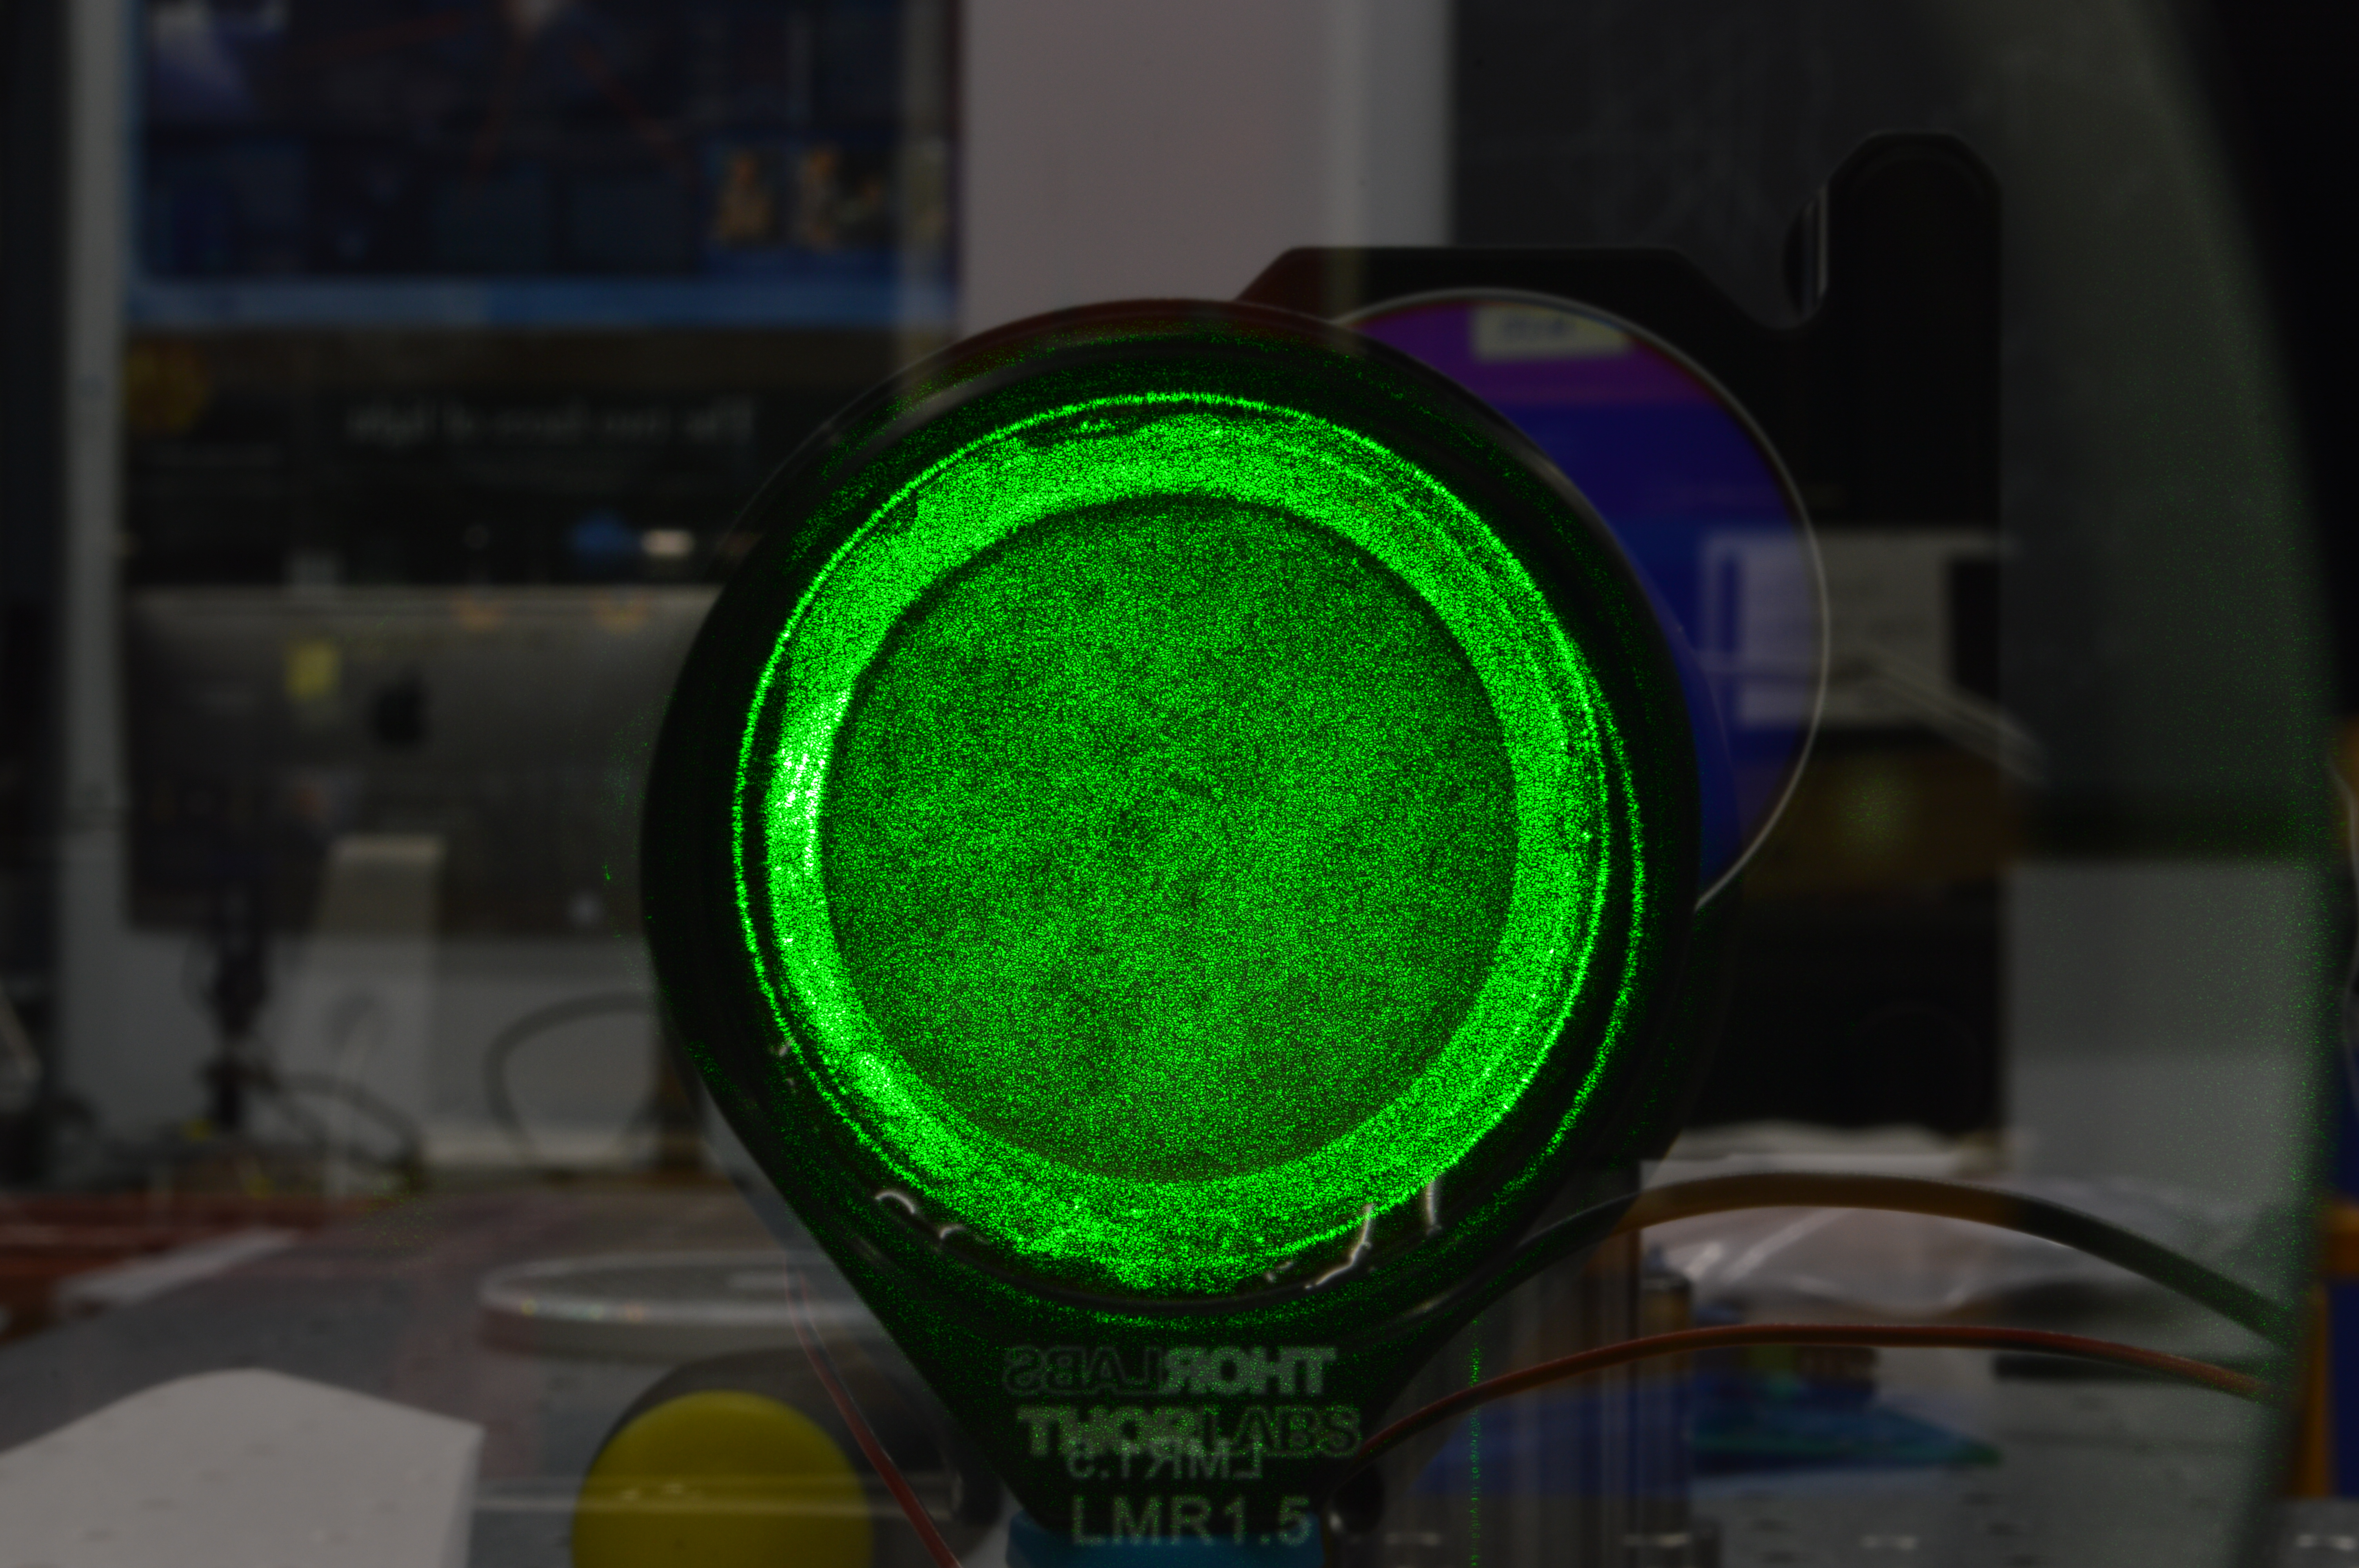
\includegraphics[width=\linewidth]{apertures/32.png}
  \caption{$a=32$}
\endminipage\hfill
\minipage{0.3\textwidth}
  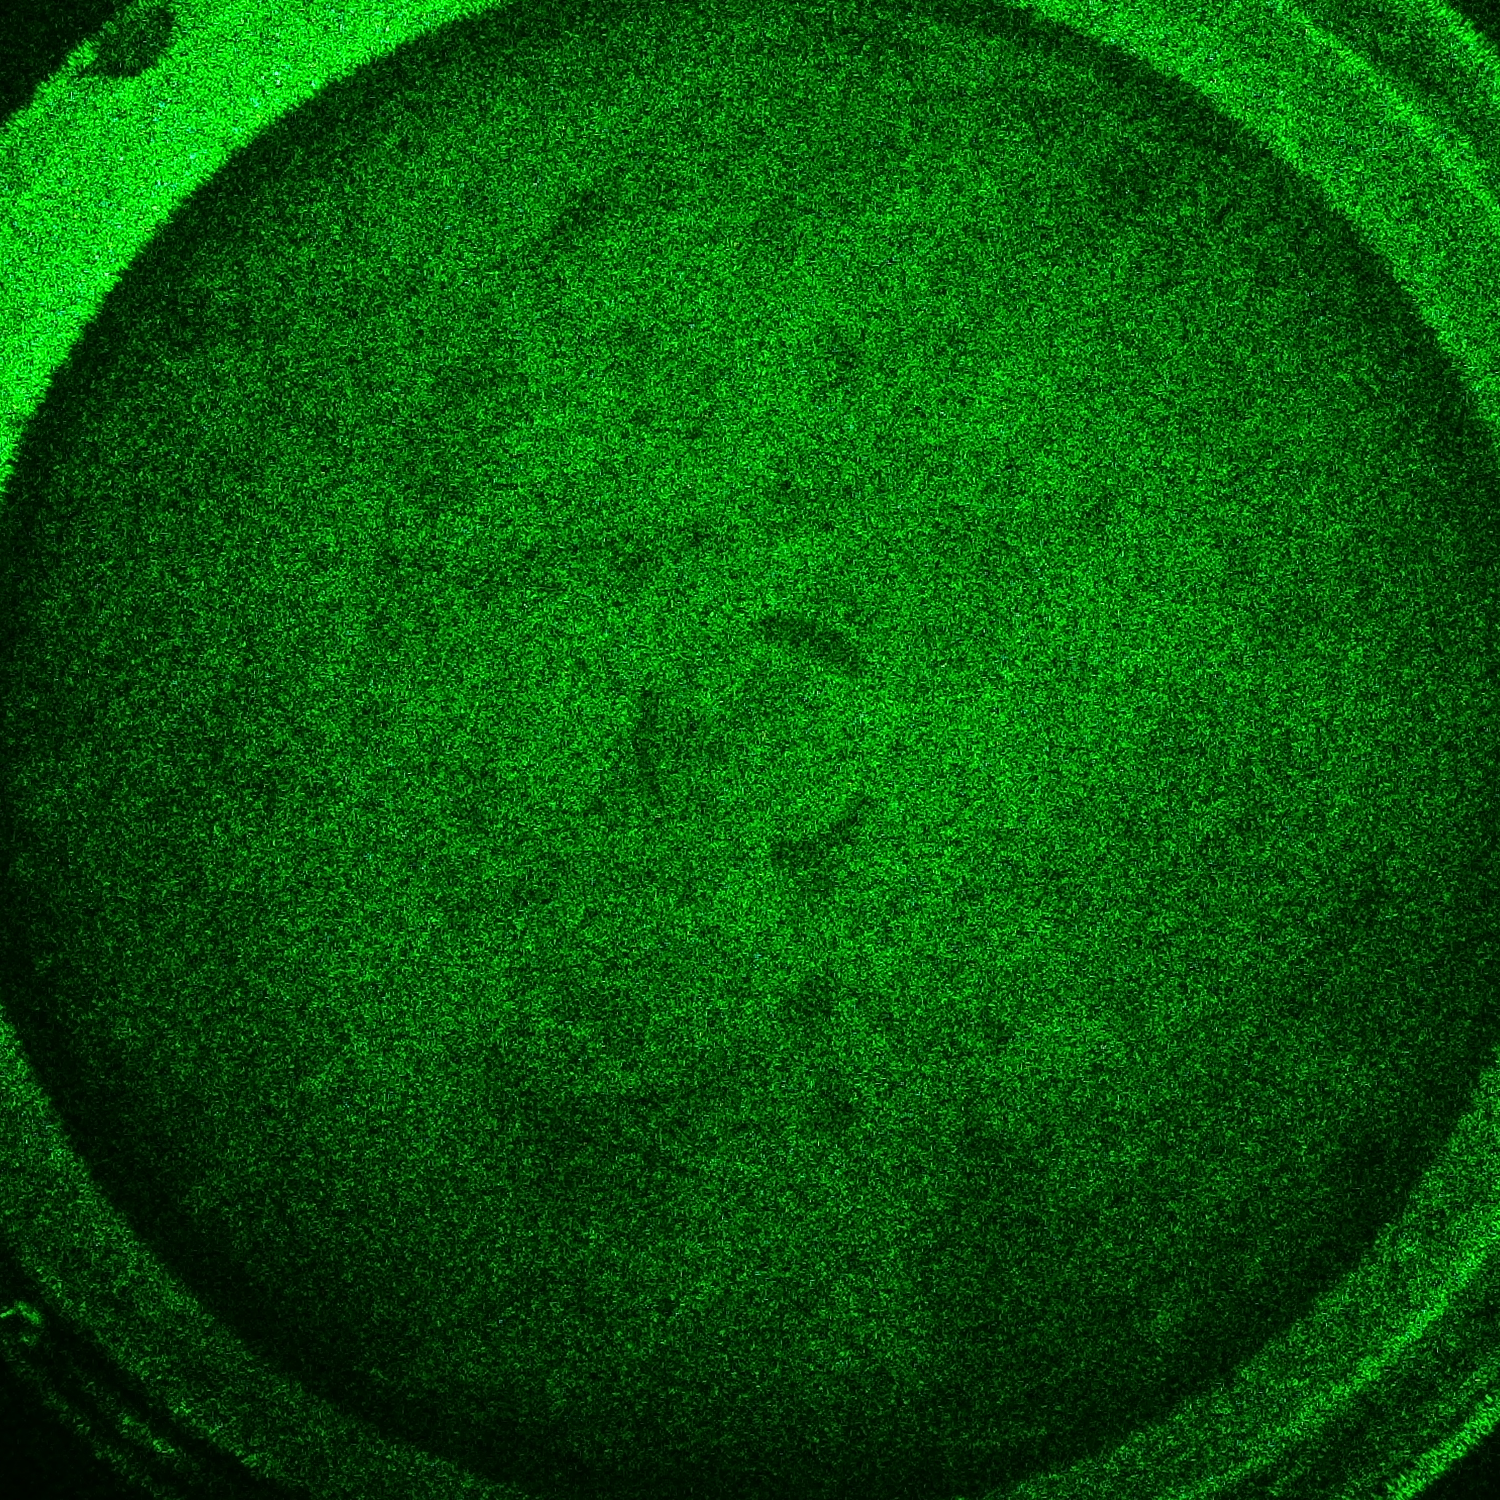
\includegraphics[width=\linewidth]{apertures/16.png}
  \caption{$a=16$}
\endminipage\hfill
\minipage{0.3\textwidth}
  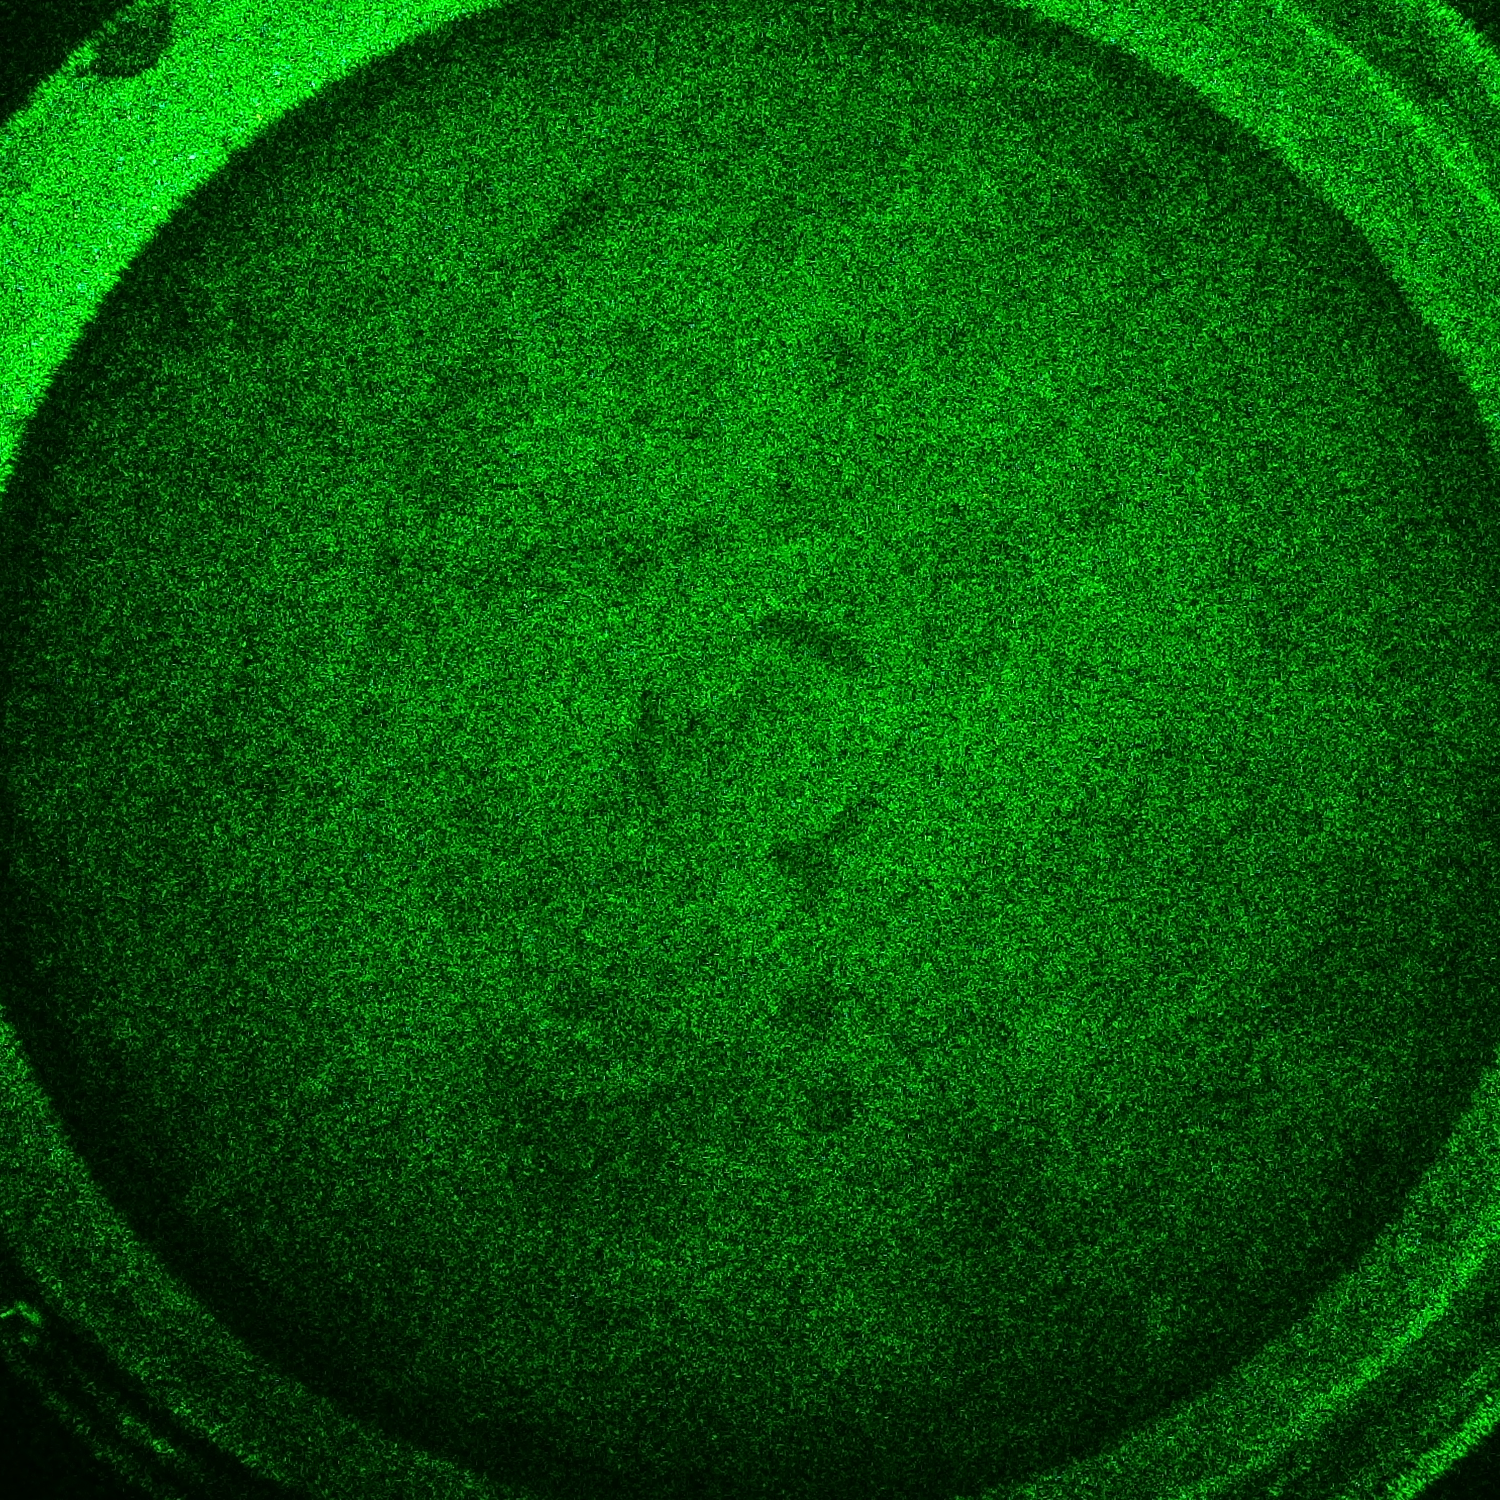
\includegraphics[width=\linewidth]{apertures/5.png}
  \caption{$a=5.6$}
\endminipage
\end{figure}
\end{frame}

\begin{frame}{Modeling Each Speckle}
We can model the intensity of each pixel via the equation$$A\cos x + b_0,$$where $A$ and $b_0$ are fixed constants, and $x$ is proportional to the distance between the aperture and the piezo at that pixel.\\
\vspace{0.5cm}
Therefore, if we translate the reference object, while holding the object of interest stationary, we would expect that the intensities of any given pixel trace out a cosine curve with some offset.
\end{frame}

\section{Setup}
\begin{frame}{Setup}
\begin{center}
  \includegraphics[width=0.4\linewidth]{diagram.png}
\end{center}
We shine the laser into a beam splitter, which sends light at both piezos, and capture the resulting speckle pattern using the camera. Each piezo is hooked up to a voltage source, which can be used to apply different voltages, causing the piezo to bulge. One piezo (the reference) has a rigid sheet attached, such that when it bulges, the entire object translates linearly with the same phase.
\end{frame}

\section{Analysis}
\begin{frame}{Calculating Absolute Phases}
\small
If we assume that we have images where the phases have shifted by exactly $\frac13$ of a wavelength, for a particular pixel, we have that
\begin{align*}
P1 &= A\cos (x)+b_0\\
P2 &= A\cos (x+2\pi /3)+b_0\\
P3 &= A\cos (x+4\pi /3)+b_0.
\end{align*}
From this, we can derive that
\begin{align*}
	A\sin(x) &= \frac{P3-P2}{\sqrt 3}\\
	A\cos(x) &= -\frac23 \left(\frac{P2+P_3}{2}-P1\right).
\end{align*}
From these two quantities it is easy to solve for $A$ and $x$.
\end{frame}

\begin{frame}{Calculating Absolute Phases}
In order to sample at exactly $\frac13$ of a wavelength, we needed to determine how the reference piezo responds to voltage.

% \vspace{.3cm}
% The interference patterns are periodic, they will repeat their patterns after the reference object has moved by exactly $\frac12$ a wavelength, corresponding to a phase shift of one wavelength. 
We did this by manually adjusting the voltage until the same pattern was seen, and recording the voltage.

\vspace{.3cm}
We found that 0.95 to 1.0 volts corresponded to a phase shift of one wavelength from the reference piezo. This can be seen in the image below, where the $x$ axis represents thirds of a volt.
% \begin{center}
% {\bf One wavelength shift}\\
% 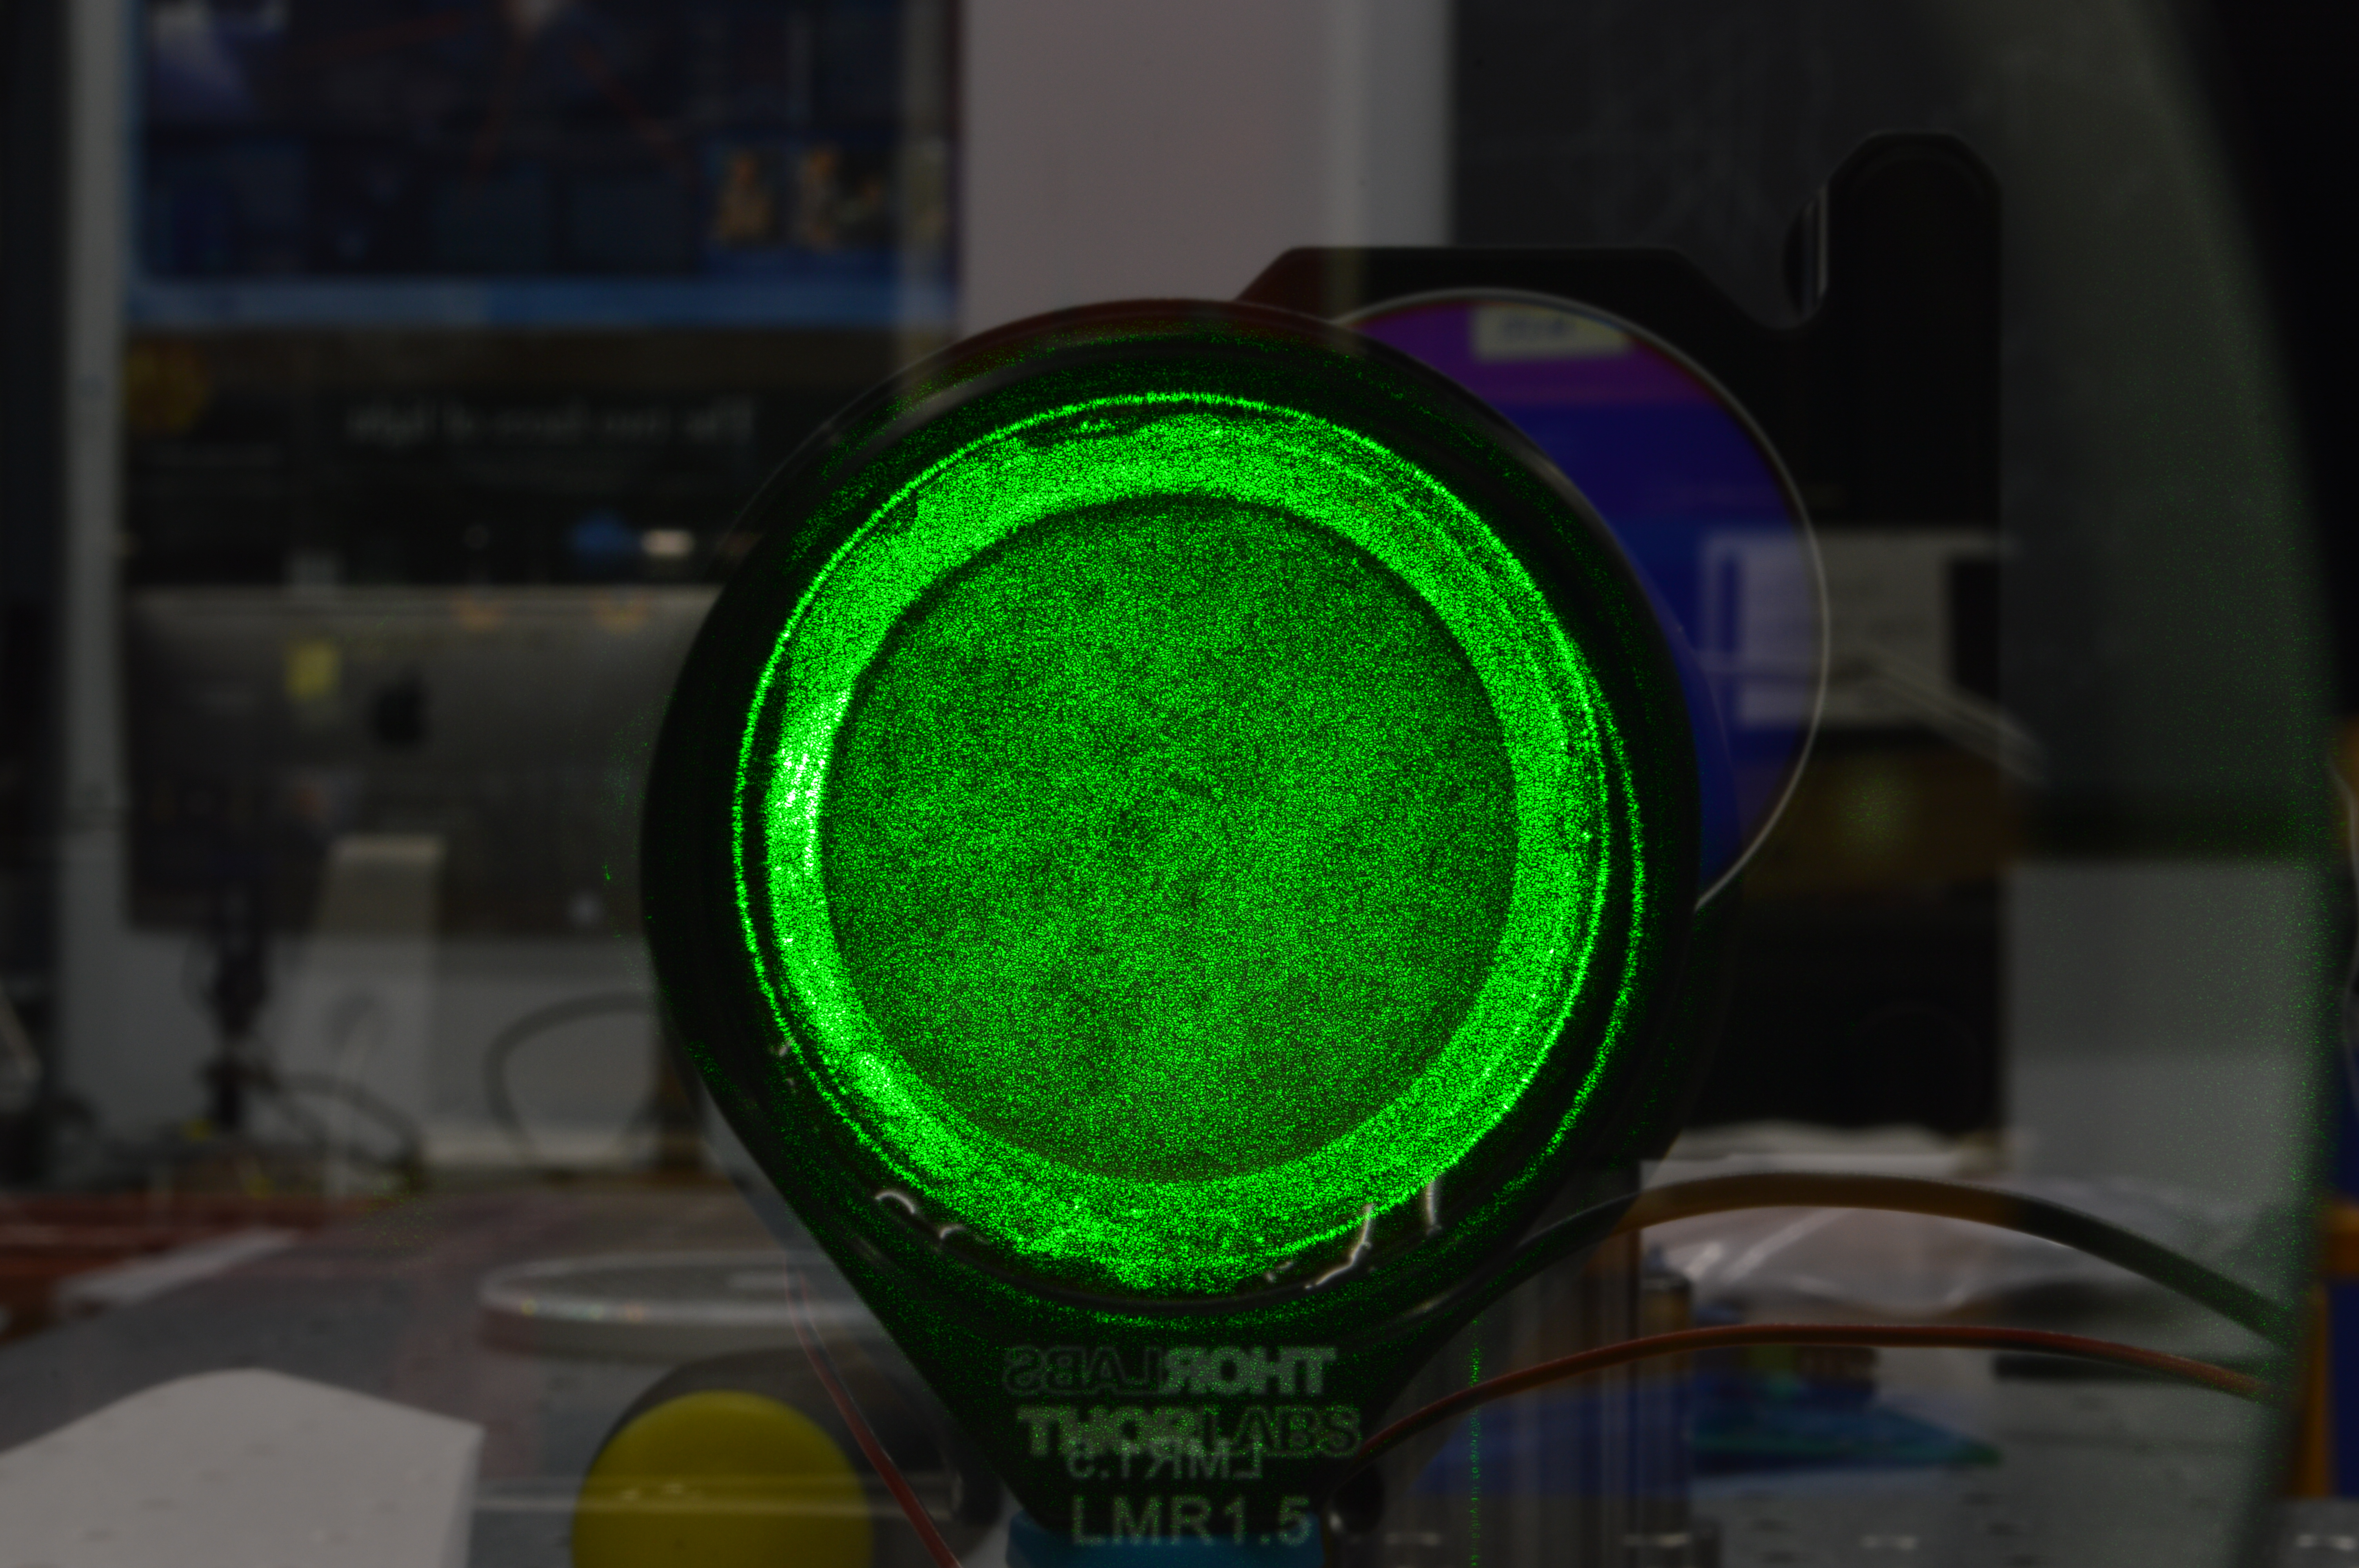
\includegraphics[width=.16\textwidth]{apertures/32.png}
% 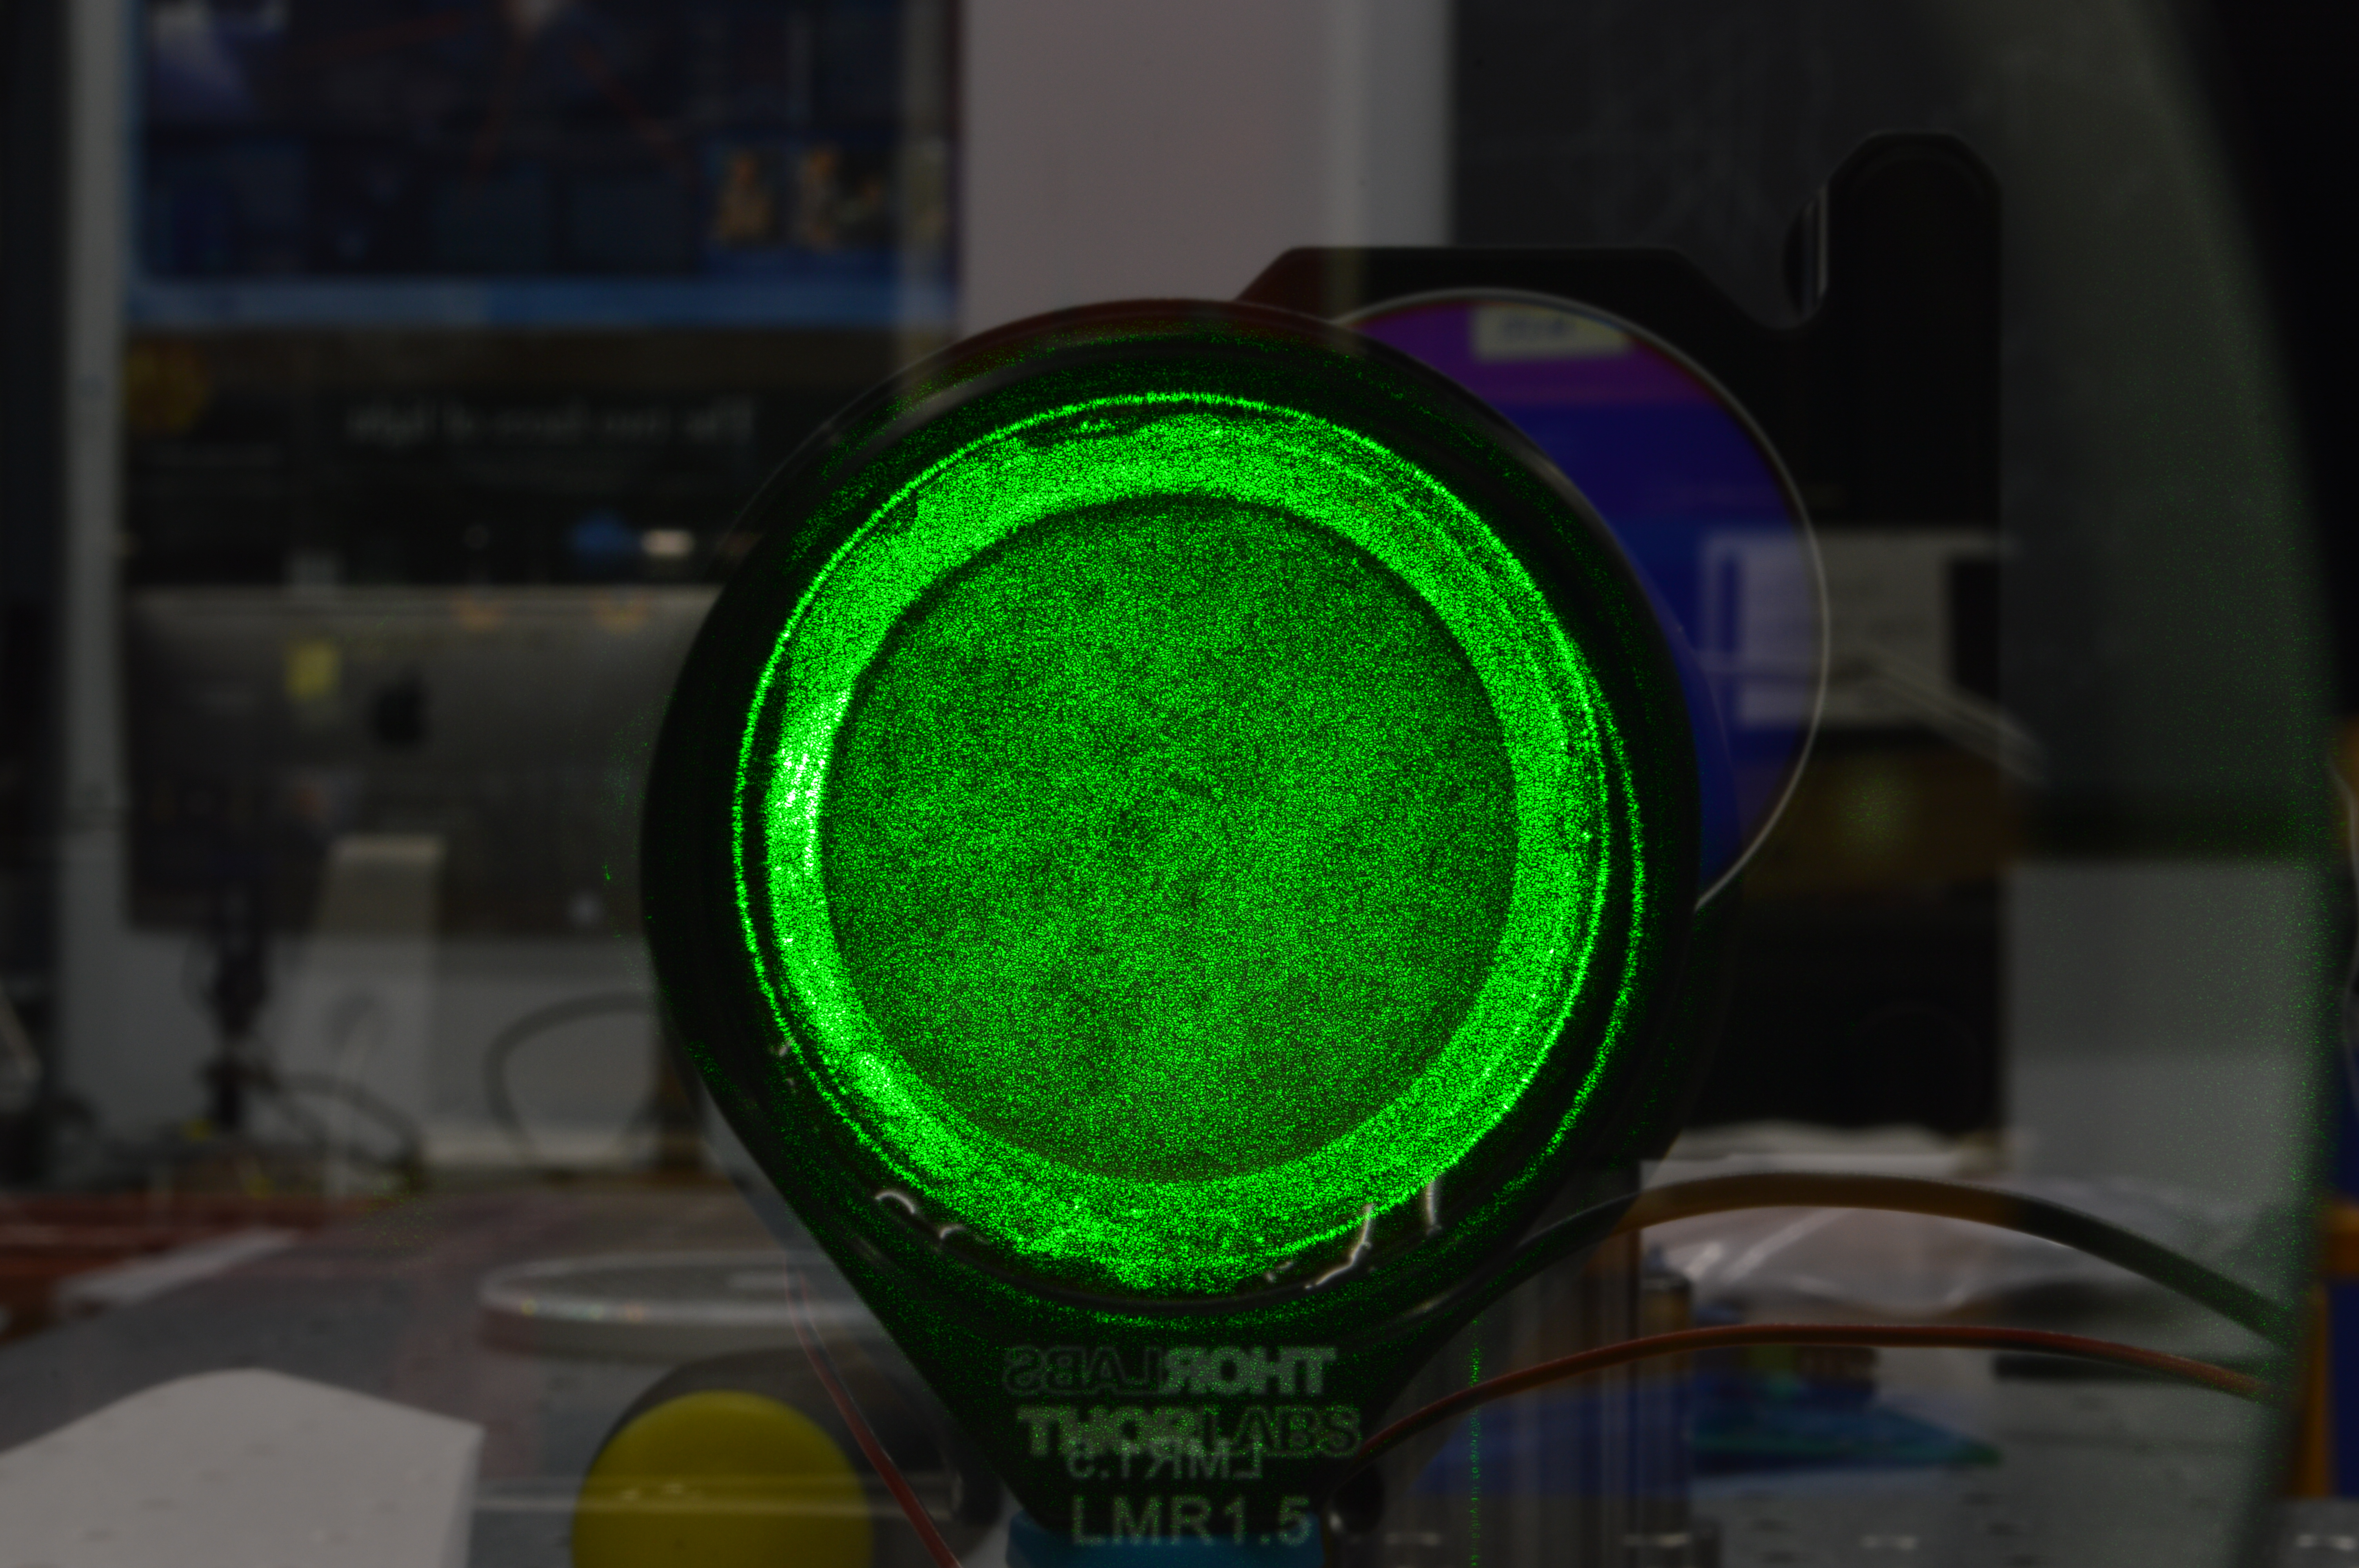
\includegraphics[width=.16\textwidth]{apertures/32.png}
% \end{center}

\begin{center}
{\bf Plot of amplitude vs voltage}
(for an arbitrary pixel)
\includegraphics[width=\textwidth]{cosine_check.png}
\end{center}

% By varying voltages at a fixed rate with our function generator, and taking pictures of the speckles at fixed intervals using the ``burst mode'' of our camera, we were able to record how the amplitude of each pixel responds to offsets in the reference object.

% Note that these points were sampled at $x = 0, \frac{2\pi}{3}, \frac{4\pi}{3},...$, which is necesary to calculate the absolute phase.
\end{frame}

\begin{frame}{Calculating Relative Phases}
We took photos of speckle patterns for the following:
\begin{itemize}
	\item piezo at 0V, varying the voltage of the reference
	\item piezo at $\frac12$V, varying the voltage of the reference
\end{itemize}
By running the absolute phase calculations for both sets of images, we were able to get phases for each pixel of each set.

\vspace{0.3cm}
Taking the differences of the absolute phases gives us a relative phase for each pixel of the image. This corresponds to how much each point on the piezo has shifted.
\end{frame}

\section{Results}
\begin{frame}{Results}

\begin{figure}[!htb]
    \centering
    \begin{minipage}{.6\textwidth}
    	\centering
		{\bf Phase shift} (brighter is closer)\\
		\includegraphics[width=\textwidth]{result.png}
    \end{minipage}~
    \begin{minipage}{0.4\textwidth}
    	This shows a bulge in the piezo by roughly half a wavelength, with the bright area corresponding to where the piezo has shifted the most.

    	\vspace{0.3cm}
        Note: to average out some of the error, we have applied a gaussian blur to the image.
    \end{minipage}
\end{figure}

\end{frame}

\section{Conclusions}
\begin{frame}{Conclusions}
The resulting image of the relative shifts is roughly what we expected, with the center of the image being brighter (larger phase shift) than the edges of the image (smaller phase shift) since the piezo is bulging outward when the voltage is applied.

\vspace{0.3cm}
We found that taking multiple images of the piezos with no voltage applied to either still showed changes in the speckle pattern. This could be the reason that the output is less than ideal. There were several sources of error that could be responsible for this:
\begin{itemize}
	\item Shifts in the camera
	\item Vibrations from the shutter
	\item Dust or changes in the temperature in the air
\end{itemize}
We were able to compensate for some of these by taking pictures in rapid succession.
\end{frame}

\section{Future Research}
\begin{frame}{Future Research}
Some additional directions in which this could be taken include:
\begin{itemize}
\item{Visualizing the behavior of membrane oscillations, by computing the relative phase differences of the surface at several moments during the oscillation.}
\item{Analyzing the stress that can be handled by a material. This could be done by applying a force, looking at the phase shifts, and looking for discontinuities that would imply cracking.}
\item{The approach itself could be improved by using more sophisticated cosine fitting algorithms to reduce the error from fitting a cosine to three points.}
\end{itemize}
\end{frame}

\section{References}
\begin{frame}{References}
\begin{itemize}
\item{\url{https://en.wikipedia.org/wiki/Speckle_pattern}}
\item{\url{https://en.wikipedia.org/wiki/Speckle_imaging}}
\item{Jacquot, P. (2008), Speckle Interferometry: A Review of the Principal Methods in Use for Experimental Mechanics Applications.}
\item{Ding, Yuan-Yuan. (2014), Image reconstruction in speckle interferometry.}
\end{itemize}
\end{frame}
\end{document}